% CHAPTER 2
\chapter{Background Knowledge}
\label{chp:background_knowledge}

\section{Perception}
\label{sec:perception}

\subsection{Human Visual System}
\label{subsec:human_visual_system}

The human visual system can be examined in three major sections : the eye, the retina and the neural structure in the brain. In this study, the main focus is the cells in the retina. These cells, named as cones, are the crucial part of the construction and the perception of the colors.

Stimulation of the cone cells has different sensitivity for each wavelength. The sensitivities of the cone cells with respect to wavelength are plotted in Figure~\ref{fig:lms_cone_normalized_sensitivities} These are the three types of cone cells, which are called with an abbreviation of their classifications according to their peak sensitive wavelengths:
\begin{itemize}
    \item $\mathbf{L}$ (Long, $\lambda_{max}$ = 565nm)
    \item $\mathbf{M}$ (Medium, $\lambda_{max}$ = 545nm)
    \item $\mathbf{S}$ (Short, $\lambda_{max}$ = 440nm)
\end{itemize}

\begin{figure}
    \centering
    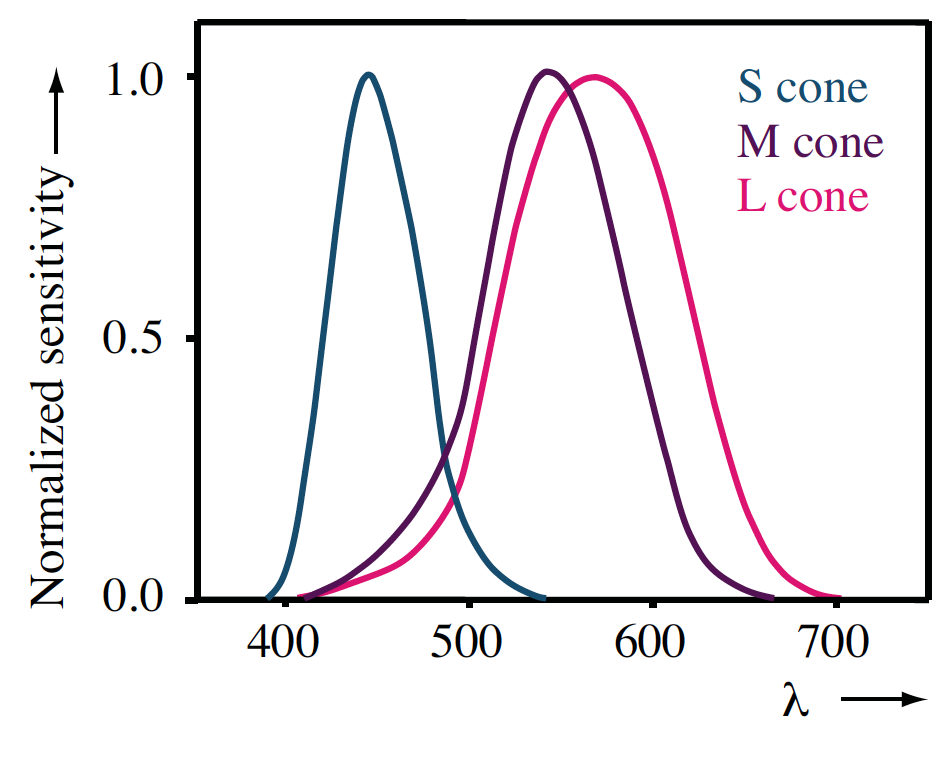
\includegraphics[width=0.5\linewidth]{figures/lms_cone_normalized_sensitivities.png}
    \caption{The normalized sensitivities of the three cone types \textit{Source:}~\cite{reinhard2008color}}
    \label{fig:lms_cone_normalized_sensitivities}
\end{figure}

\subsection{Reflectance and Illumination}
\label{subsec:reflectance_and_illumination}

A light can interact with an object in three ways: absorption, transmission and reflection. Every material has its own absorption, transmission and reflection function with respect to wavelength that sum to unity due to the conservation of energy. Absorbed, transmitted and reflected spectrum of light is just the multiplication of the spectrum of light with the material's absorption, transmission and reflection functions respectively.

Only the transmitted and reflected light can be perceived by human sensory system as the light incidents to the retina cells. Transmitted light is generally omitted or considered as reflected light in the study of chromatic adaptation. As a result, we will express the incident light $\mathbf{E}(\lambda)$ in the Eq.~\ref{eq:incident_light_formula} as the multiplication of the light function $\mathbf{I}(\lambda)$ and the material's reflection function $\mathbf{R}(\lambda)$ where $\lambda$ is the wavelength and it belongs to the visible spectrum $\mathbf{\Lambda}$. The visual representation of this equation is showed in Figure`\ref{fig:reflection_and_illumination}.

\begin{equation}
\mathbf{E}(\lambda) = \mathbf{I}(\lambda) \mathbf{R}(\lambda), \lambda \in \mathbf{\Lambda}
\label{eq:incident_light_formula}
\end{equation}

\begin{figure}
    \centering
    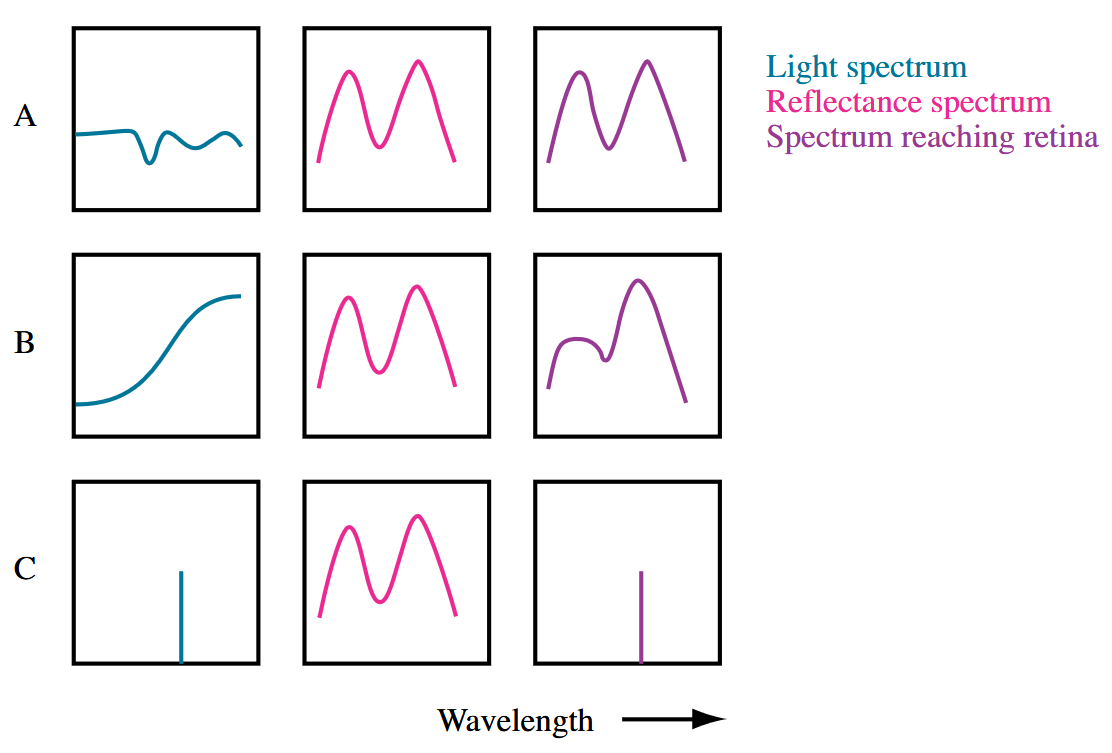
\includegraphics[width=0.8\linewidth]{figures/reflection_and_illumination.png}
    \caption{Visual representation of the multiplication of the light and the material's reflectance function in the Eq.~\ref{eq:incident_light_formula} \textit{Source:}~\cite{reinhard2008color}}
    \label{fig:reflection_and_illumination}
\end{figure}

\subsubsection{Dichromatic Reflection Model}
\label{sec:dichromatic_reflection_model}
Dichromatic reflection model analyzes the path of the reflected light in detail. The model separates the reflected light into two components: specular reflection and diffuse reflection.

The light that is immediately reflected after interacting with the material is not absorbed by the material. This type of light carries the information about the light source and it is named as specular reflection. The light that enters the object, exits from the surface without being absorbed by the object and scatters in every direction carries the information about the material and it is named as diffuse reflection. Therefore, the incident light to the retina carries the information of both and the incident light to retina model explained in Eq.~\ref{eq:incident_light_formula} is updated as Eq.~\ref{eq:dichromatic_incident_light_formula} where $\mathbf{R}_s(\lambda)$ and $\mathbf{R}_d(\lambda)$ represents the specular reflection and diffuse reflection respectively.

\begin{equation}
\mathbf{E}(\lambda) = \mathbf{I}(\lambda) (\mathbf{R}_s(\lambda) + \mathbf{R}_d(\lambda)), \lambda \in \mathbf{\Lambda}
\label{eq:dichromatic_incident_light_formula}
\end{equation}

Decomposing the terms $\mathbf{R}_s(\lambda)$ and $\mathbf{R}_d(\lambda)$ becomes important from the perspective of the study of illumination estimation.

\subsection{Camera Model}
\label{subsec:camera_model}

Modern digital cameras have three major components: the lens, the sensor and the image signal processor. The focus of this study covers the sensor and white balance correction step in the pipeline of image signal processing.  White balance correction step is explained in more detail in the following section \ref{sec:chromatic_adaptation_and_white_balance} of this chapter. The sensor is the crucial part where the light is captured for each of its primitive color components as energy and converted into electric current. The formula of the camera sensor model is given in Eq.~\ref{eq:camera_model_formula}. The incident light is filtered by proper color of the color filter array and then the light interacts with the sensor material, which generates electric current depending on its quantum efficiency with respect to the wavelength of the light.

The term $I_c$, an integration of the multiplication of some spectral distribution functions on the visible spectrum, represents the pixel value of the channel $c$ where $c \in \{R,G,B\}$ and $R,G,B$ are the abbreviations of the primary colors of the color filter array: red, green and blue. $\mathbf{E}(\lambda)$ represents the total energy of the incident light with respect to wavelength during the exposure which is explained in the Eq.~\ref{eq:incident_light_formula} in the section~\ref{subsec:reflectance_and_illumination}. $\mathbf{C}_c(\lambda)$ represents the transmitting proportion of the related filter of the color filter array with respect to wavelength. $\mathbf{Q}(\lambda)$ represents the quantum efficiency of the sensor material with respect to wavelength. Generally, the multiplication of $\mathbf{C}_c(\lambda)$ and $\mathbf{Q}(\lambda)$ is unique for every camera sensor and considered as a single component of the equation that is showed as $\mathbf{S}_c(\lambda)$ where $S$ represents the sensor sensitivity for the channel $c$. Finally, expanding the equation of $\mathbf{E}(\lambda)$, we acquire the core equation (Eq.~\ref{eq:camera_model_formula_sensor_sensitivity}) that will be used through this study.

\begin{subequations}
\label{eq:camera_model_formula}
\begin{align}
I_c = \int_{\mathbf{\Lambda}} \mathbf{E}(\lambda) \mathbf{C}_c(\lambda) \mathbf{Q}(\lambda) \, d\lambda \label{eq:camera_model_formula_separated} \\
I_c = \int_{\mathbf{\Lambda}} \mathbf{E}(\lambda) \mathbf{S}_c(\lambda) \, d\lambda \label{eq:camera_model_formula_sensor_sensitivity} \\
I_c = \int_{\mathbf{\Lambda}} \mathbf{I}(\lambda) \mathbf{R}(\lambda) \mathbf{S}_c(\lambda) \, d\lambda \label{eq:camera_model_formula_pixel}
\end{align}

\end{subequations}

\section{Chromatic Adaptation \& White Balance}
\label{sec:chromatic_adaptation_and_white_balance}

The color of the illuminant hitting the surface changes the observed color of the surface in a non-decomposable manner as can be derived from the section~\ref{subsec:reflectance_and_illumination}. However, human visual system can identify the object and its color under different lighting conditions by naturally removing the effect of the light source. This is known as color constancy~\cite{reinhard2008color}. In a specific manner, a white surface appears white to the human visual system under different light conditions as well. White balance is defined as the process of replicating this adaptation of human perception. 

\section{von Kries Coefficient Law}
\label{sec:von_kries_coefficient_law}

Johannes von Kries, in 1878, introduced a linear chromatic adaptation formula, as known as von Kries Coefficient Law, that is still used as an effective way of correcting the white balance. As explained in detail by MacAdam~\cite{MacAdamChromaticAdaptationVonKriesExplained1981}, von Kries defines the adaptation process as a multiplication of cone responses with a gain factor. In addition, this process becomes more coherent with the idea of independent channel adaptation. As a result, we obtain a linear diagonal transformation in the Eq.~\ref{eq:von_kries_lms}.

\begin{equation}
    \begin{bmatrix} 
    L_c \\ 
    M_c \\ 
    S_c 
    \end{bmatrix} = 
    \begin{bmatrix} 
    \alpha & 0 & 0 \\ 
    0 & \beta & 0 \\ 
    0 & 0 & \gamma 
    \end{bmatrix} 
    \begin{bmatrix} 
    L \\ 
    M \\ 
    S 
    \end{bmatrix}
    \label{eq:von_kries_lms}
\end{equation}

$L_c,M_c,S_c$ are the adapted cone responses with the coefficients $\alpha, \beta, \gamma$. The law states that the observer can see the object as the object is under an other light source if the per channel sensor response ratio is multiplied with the sensor response of the reflected light from the object. The statement is explained as an equation in Eq.~\ref{eq:von_kries_statement}.

\begin{equation}
    \begin{bmatrix} 
    L_2 \\ 
    M_2 \\ 
    S_2 
    \end{bmatrix} = 
    \begin{bmatrix} 
    \frac{L_2}{L_1} & 0 & 0 \\ 
    0 & \frac{M_2}{M_1} & 0 \\ 
    0 & 0 & \frac{S_2}{S_1} 
    \end{bmatrix} 
    \begin{bmatrix} 
    L_1 \\ 
    M_1 \\ 
    S_1 
    \end{bmatrix}
\label{eq:von_kries_statement}
\end{equation}

The terms $L_1, M_1, S_1$ represents the per channel sensor responses from the reflected light from the object with an arbitrary light. The terms $L_2, M_2, S_2$ represents the per channel sensor responses from the reflected light from the object with an other arbitrary light.

This equation explains that how the cells in retina adapt to the new light source and preserve the observed chromaticity of the object under different light sources by applying gain coefficients per channel.

\subsection{Wrong von Kries}

The camera model explained in the section~\ref{subsec:camera_model} has its own sensor response functions per channel which are being aimed to be identical with the cone cells but are not able to be exactly identical due to industrial reasons. In addition, white balance correction procedure is applied on the linear raw image data which the color space is the sensor's color space in the image signal processing pipeline. These enforce us to apply von Kries Coefficient Law on a different color space rather than LMS color space where the method is truly valid. This application is named as "wrong von Kries" as explained in~\cite{reinhard2008color} and formulated as in the Eq.~\ref{eq:wrong_von_kries_rgb}.

\begin{equation}
    \begin{bmatrix} 
    R_c \\ 
    G_c \\ 
    B_c 
    \end{bmatrix} = 
    \begin{bmatrix} 
    \alpha & 0 & 0 \\ 
    0 & \beta & 0 \\ 
    0 & 0 & \gamma 
    \end{bmatrix} 
    \begin{bmatrix} 
    R \\ 
    G \\ 
    B 
    \end{bmatrix}
    \label{eq:wrong_von_kries_rgb}
\end{equation}

The terms $R_c,G_c,B_c$ and $R,G,B$ represent the corrected RGB color channel values and the original RGB color channel values respectively. The illumination estimation works explained in the following chapters~\ref{chp:related_works} and~\ref{chp:proposed_method} aim to find the coefficients $\alpha$, $\beta$ and $\gamma$ in the sensor's color space for white balance correction.